\documentclass[10pt, aspectratio=169]{beamer}
\usepackage{beamerthemeMathFest}
\usepackage{tcolorbox}

\title[MaxEnt Models]{Applying Maximum Entropy Models to Organism Sensors}
\vspace{1em}
\subtitle{MAA MathFest 2026, Boston}
\author{Christopher Wang}
\institute{Scripps College}
\date{August 7, 2026}

\graphicspath{figs/}

\begin{document}

\maketitle

\begin{frame}{Outline}
\tableofcontents
\end{frame}

\section{Acknowledgements}

\begin{frame}{Acknowledgements}
	\begin{itemize}\addtolength{\itemsep}{10pt}
		\item PI: Sarah Marzen
		\item Co-authors: Eliana Schimke, Martina Lamberti, Joost le Feber, Tristan Kako, Sarah Marzen
	\end{itemize}
\end{frame}

\section{Introduction}

\begin{frame}{Motivation}

\begin{columns}
	\begin{column}{0.62\textwidth}
		\textbf{\textcolor{red!60!black}{How do biological organisms understand their enviornment?}}
		\pause
		\vspace{1em}
		\begin{enumerate}\addtolength{\itemsep}{10pt}
			\item Encodes information about enviornment
			\item Past, present, and future
			\item Constraint: energetic cost of encoding
		\end{enumerate}
	\end{column}
	\begin{column}{0.35\textwidth}
		\begin{figure}
			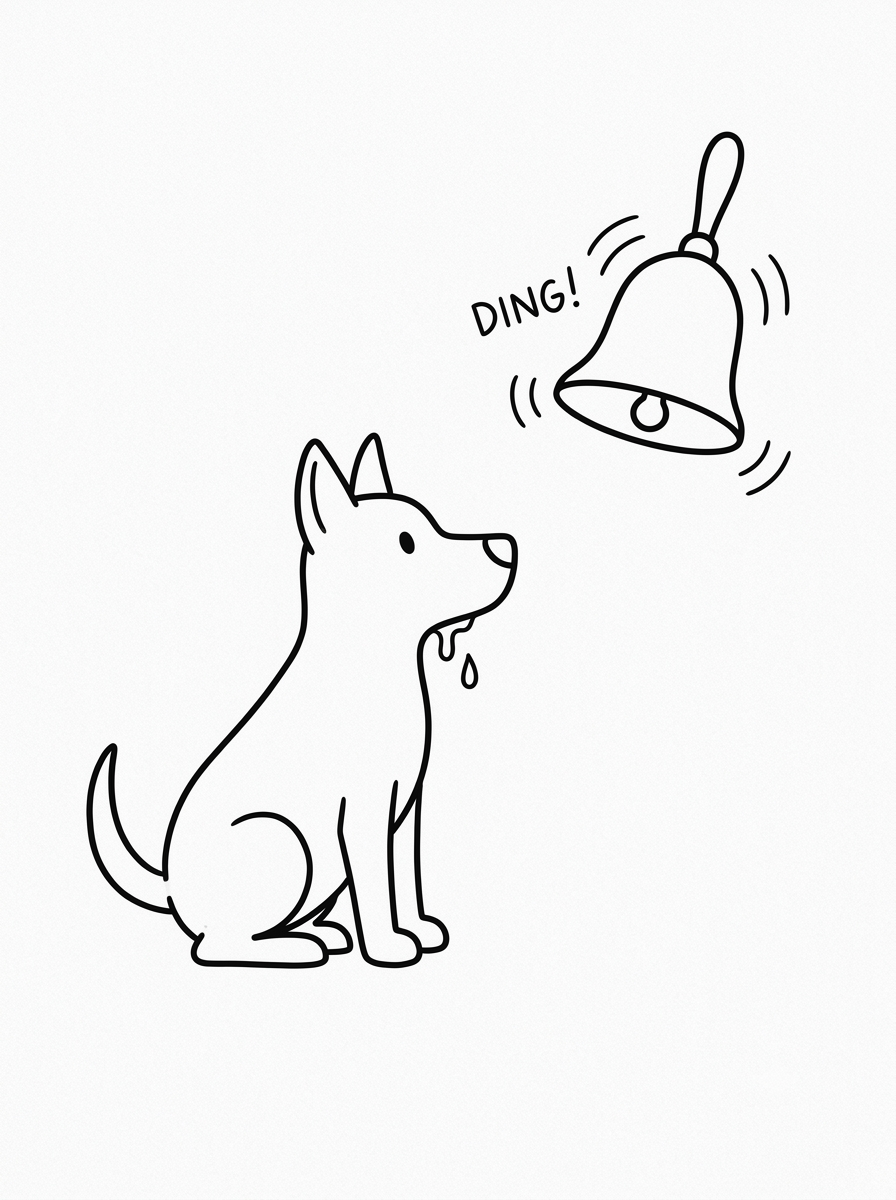
\includegraphics[width=0.9\textwidth]{figs/pavlov dog.png}
		\end{figure}
	\end{column}
\end{columns}
\end{frame}


\begin{frame}{Entropy: a Fundamental Player}

\vspace{1em}

\begin{center}
	\textbf{How well can we encode/compress information?}	
\end{center}

\vspace{1em}

\begin{block}{Shannon Entropy}
	For a random variable $X$ and event space $\mathcal{X}$,
\begin{equation}
	H[X] = -\sum_{x \in \mathcal{X}} p(x) \log_b(p(x)),
\end{equation}
where $b=2,e,10$ most commonly. 
\end{block}
\end{frame}

\begin{frame}{Entropy: a Fundamental Player}

\begin{columns}
	\begin{column}{0.65\textwidth}
	\begin{exampleblock}{Flipping Coins ($b=2$)}
		Entropy of one fair coin flip ($C$) and one biased ($B,~p_\text{heads}=0.7$):
	\begin{align}
		H[C] &= -\sum_{x \in \mathcal{X}} p(x) \log_b(p(x)) = -\log_2(1 / 2) = 1 \text{ bit.} \\
		H[B] &= -0.7\log_2(0.7) -0.3\log_2(0.3) \approx 0.88 \text{ bits.}
	\end{align}
	\pause
		Entropy of flipping two fair coins ($C_1, C_2$):
	\begin{equation}
		H[C_1, C_2] = -\log_2(1 / 4) = H[C] + H[C] = 2 \text{ bits.}
	\end{equation}
	\pause
		Entropy of flipping two coins and adding them ($C_1+C_2$):
	\begin{equation}
		H[C_1+C_2] = 1.5 \text{ bits.}
	\end{equation}
\end{exampleblock}
	\end{column}
	\hfill
	\pause
	\begin{column}{0.3\textwidth}
		Key takeaways:
		\vspace{10pt}
		\begin{itemize}\addtolength{\itemsep}{10pt}
			\item $H[X, Y] \le H[X] + H[Y]$, equality if $X, Y$ ind.
			\item ``Surprisal": $-\log p$
			\item \textcolor{red!80!black}{Maximum entropy minimizes surprisal}
		\end{itemize}
	\end{column}
\end{columns}


\end{frame}

\begin{frame}{Mutual Information: One Take on Entropy}
	\begin{tcolorbox}[colback=red!20!white, arc=2mm, colframe=red!60!black]
		How much information do I gain about the environment by analyzing a biological sensor system?
	\end{tcolorbox}
	\begin{equation}
		I[S; X] = H[S] - H[S \mid X]
	\end{equation}
\end{frame}

\begin{frame}{Shortcomings with Mutual Information}
	\begin{itemize}
		\item Hard to calculate
		\item Only one metric
	\end{itemize}
\end{frame}

\begin{frame}{Maximum Entropy: An Alternate Lens}
	\begin{itemize}
		\item Given constraints, maximize $H[X]$.
		\item Lagrange Multiplier problem (illustrate)
		\item Quantify performance: using bias/var and confusion matrices
		\item Lots of info
	\end{itemize}
\end{frame}


\section{Conclusion}
{\BackgroundShaded
\begin{frame}
\begin{center}
	Thank you!
\end{center}
\end{frame}}

\end{document}
